\documentclass[12pt]{article}

\usepackage[utf8]{inputenc}
\usepackage[T1]{fontenc}
\usepackage[french]{babel}
\usepackage[hidelinks]{hyperref}
\usepackage{graphicx}
\usepackage{amsmath}


\title{Bataille Navale}
\author{Damien MARIS, Evens ANTOINE, Boubacar Sadio DIALLO, Alain David BERIMANA}
\date{14 Avril 2023}

\begin{document}
\maketitle
\thispagestyle{empty}
\newpage
\clearpage
\pagenumbering{arabic} 
\tableofcontents
\newpage
\section{Introduction}
Voici notre rapport sur le projet Bataille Navale conçu en MVC par ANTOINE Evens, BERIMANA Alain David, DIALLO Boubacar Sadio et MARIS Damien.



\section{Jouabilité}

\subsection{Bataille Navale Console}
\begin{figure}[h]
\center
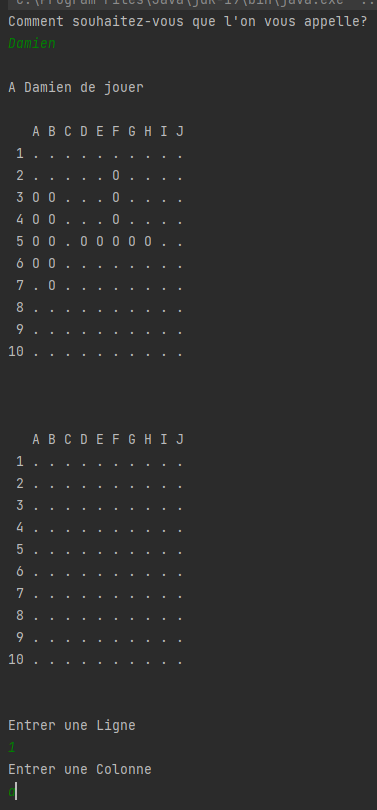
\includegraphics[width=0.2\textwidth]{./images/debutPartieConsole.png}
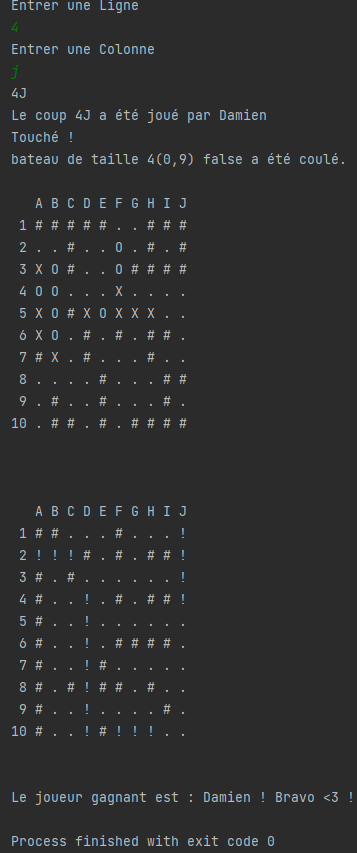
\includegraphics[width=0.2\textwidth]{./images/finPartieConsole.png}
\caption{affichage d'une partie en Console\label{img:figure1}}

\end{figure}
Dans la figure \ref{img:figure1} nous avons un aperçu de l'affichage de la grille. Pour mieux nous allons expliciter les symboles :
\begin{itemize}
    \item Le symbole "\textbf{.}" montre qu'aucun tir n'a été effectué dans cette case.
    \item Le symbole "\textbf{O}" montre une pièce de bateau intacte.
    \item Le symbole "\textbf{X}" montre qu'une pièce de bateau a été touchée.
    \item Le symbole "\textbf{\#}" montre que le tir a été loupé.
    \item Le symbole "\textbf{!}" montre qu'une pièce de bateau a été coulée. Ce symbole apparaît donc une fois que tout le bateau a été coulé.
    
\end{itemize}
Le premier joueur commence et doit mettre son nom dans la console. Ensuite il est amené à entrer une ligne jouable toujours dans la console puis il doit saisir la colonne sous forme de caractère. Si la saisie est incorrecte, le joueur est amené à recommencer à choisir son coup. Ensuite l'ordinateur s'occupe de jouer son coup et tout ceci recommence tant que l'une des flottes n'est pas coulée entièrement.
\subsection{Bataille Navale Graphique}
\begin{figure}[h]
\center
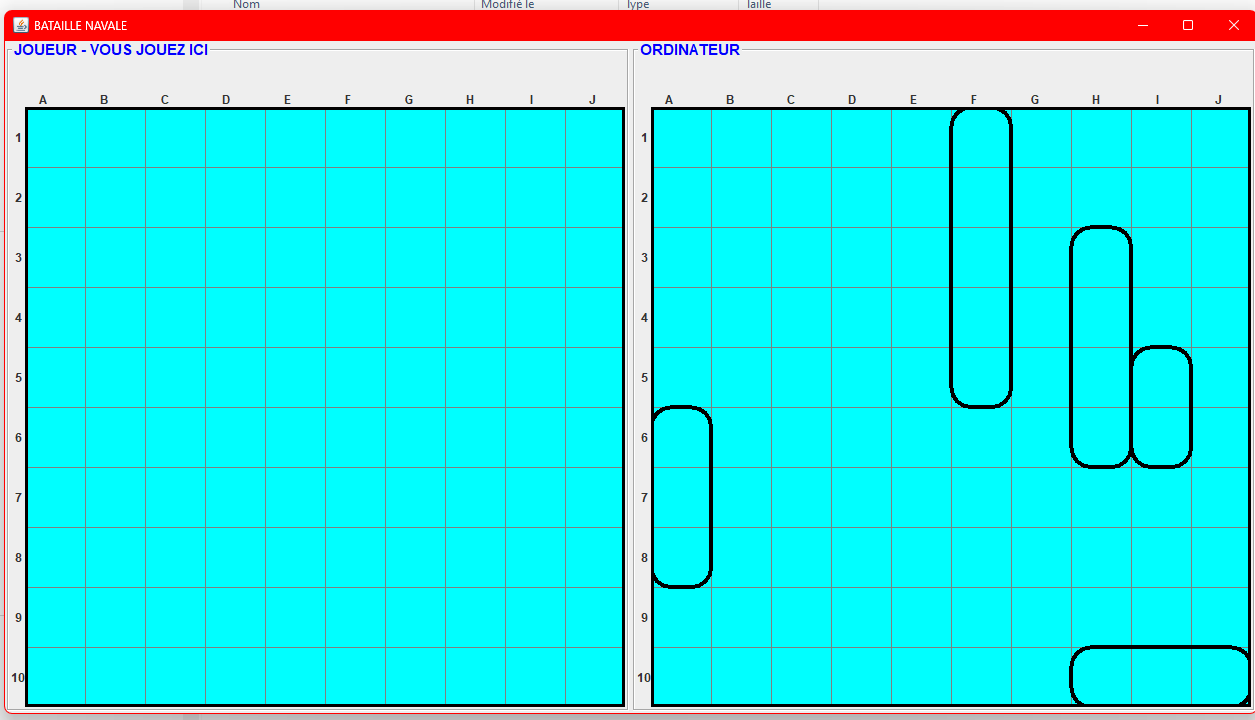
\includegraphics[width=0.4\textwidth]{./images/debutPartieGr.png}
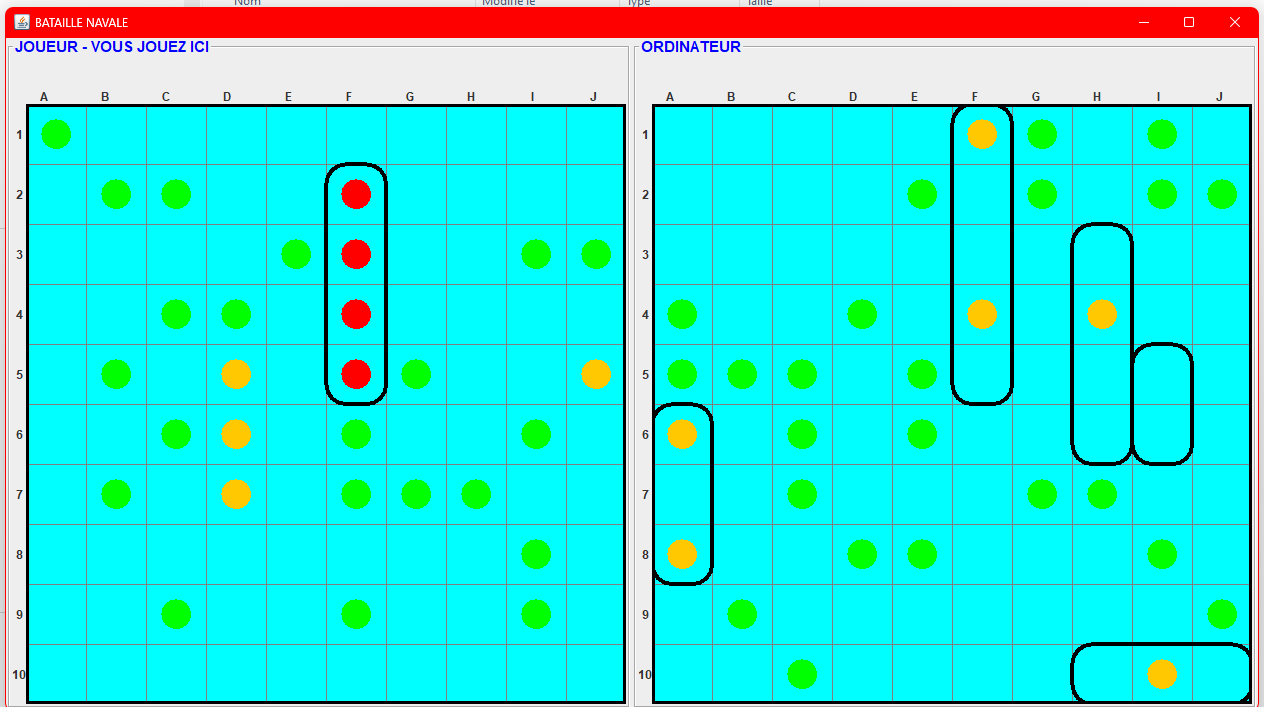
\includegraphics[width=0.4\textwidth]{./images/milieuPartieGra.png}
\caption{affichage d'une partie en Interface Graphique(début et milieu)\label{img:figure2}}
\end{figure}

\begin{figure}[h]
\center

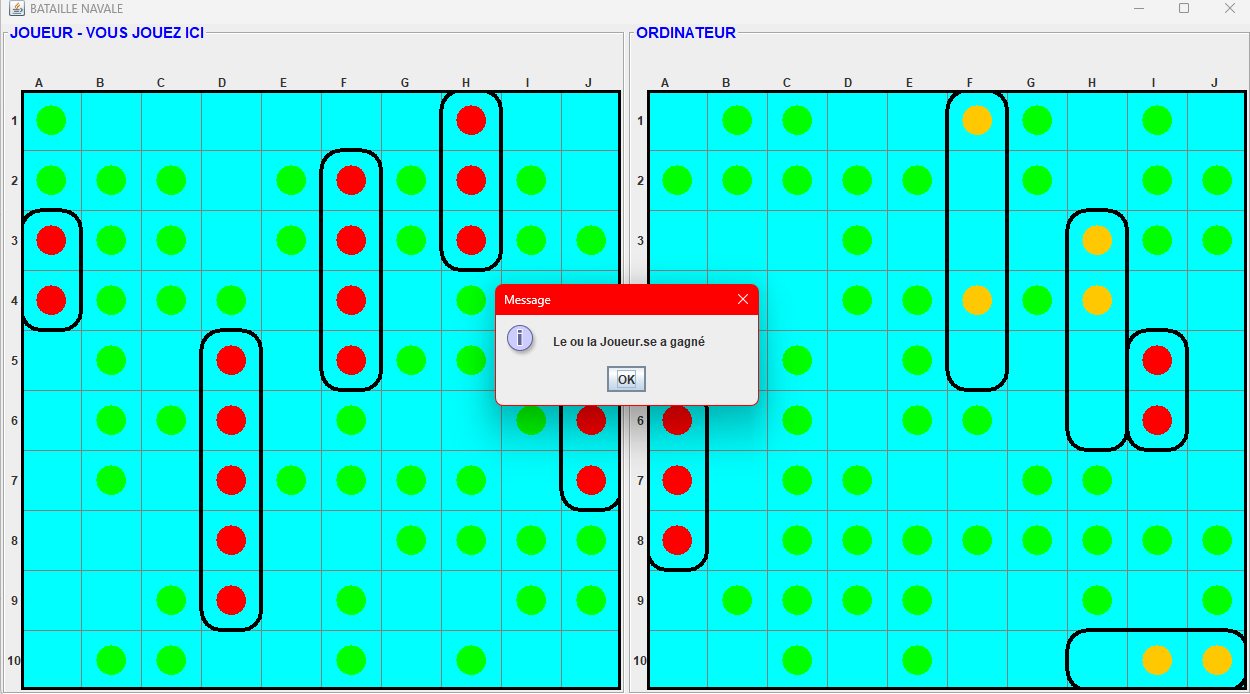
\includegraphics[width=0.4\textwidth]{./images/finPartieGraphique.png}
\caption{affichage d'une partie en Interface Graphique(fin)\label{img:figure2}}
\end{figure}

Les bateaux sont entourés en noir. Quand une pièce de bateau est touché, la pièce se colorie en orange. Si tout un bateau est coulé, l'entourage du bateau est dévoilé et toutes les pièces se colorient en rouge. Si on loupe le tir, la case est coloriée en vert.
Les cases cliquables sont celles de gauche, le joueur clique sur une case puis automatiquement, un coup est joué sur la grille de droite qui est notre grille, celle où l'ordinateur joue.
Tout ceci s'arrête quand toute la flotte d'un joueur (ordinateur ou utilisateur) a été décimée et la fenêtre se ferme.

\section{Explications}
\subsection{Diagramme des classes}

\begin{figure}[ptbh]
\center

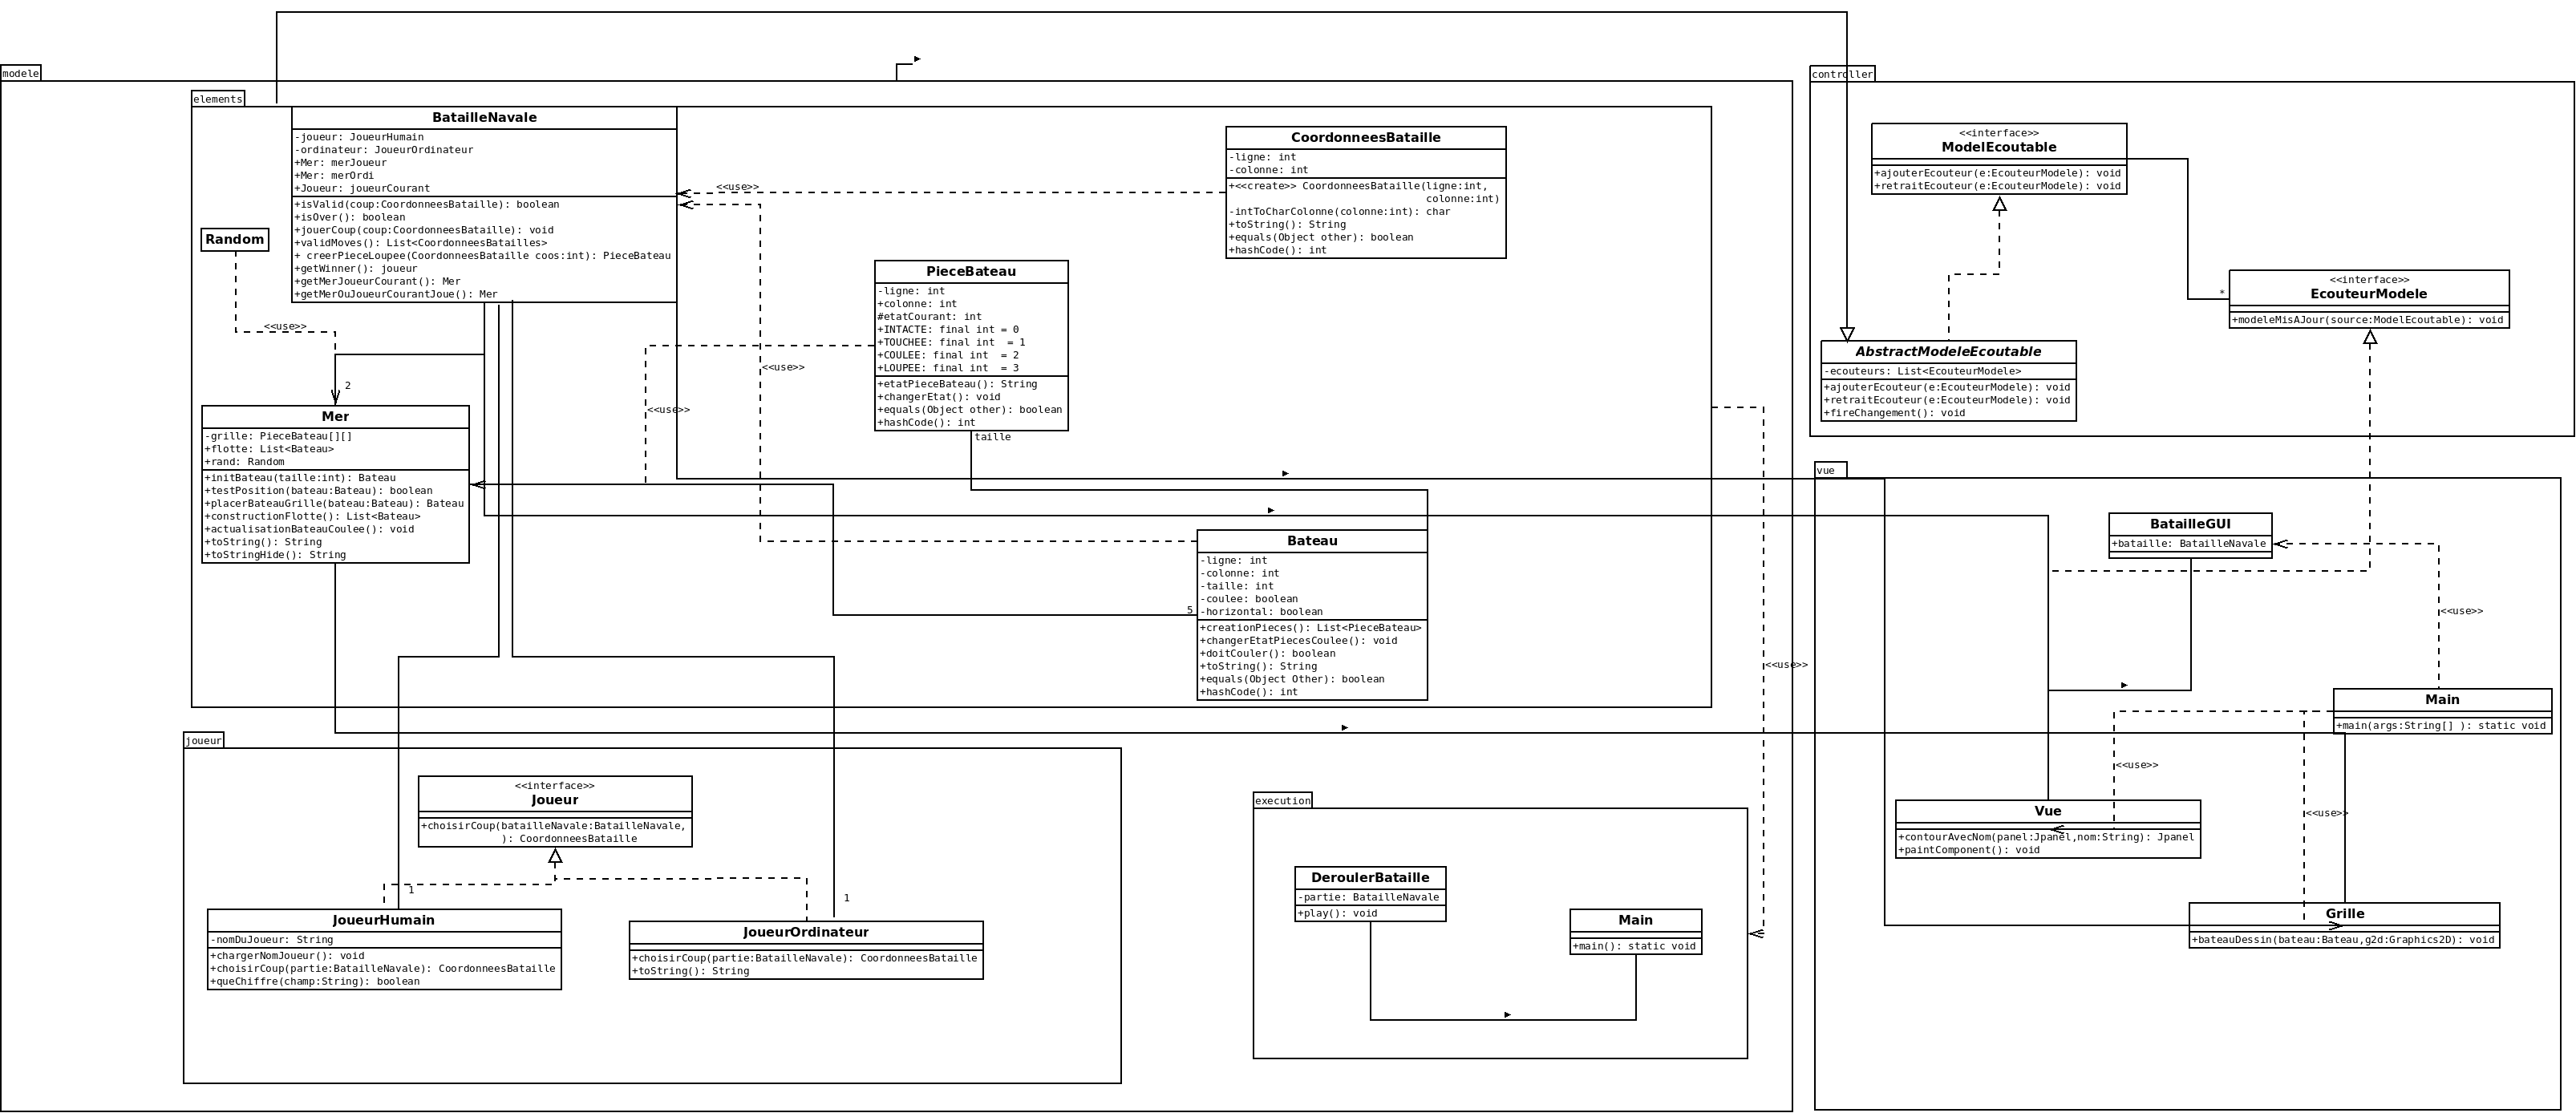
\includegraphics[width=1\textwidth]{./images/diagrame.png}
\caption{diagramme des classes\label{img:figure2}}
\end{figure}
Organisation des packages:
\begin{itemize}
    \item src \begin{itemize}
    				\item modele \begin{itemize}
    								\item execution
    								\item elements
    								\item joueurs
    							\end{itemize}
    				\item controller
    				\item vue
    			\end{itemize}
\end{itemize}

\subsection{Points a spécifier du code}
Le package modele.elements contient les éléments qui sont propre à la construction de Bataille Navale. Les voici:
\begin{itemize}
	\item La classe BatailleNavale contenant les règles d'une bataille navale
	\item La classe Bateau qui créer un objet bateau alimentant la flotte d'un joueur
	\item La classe PieceBateau qui est la classe servant à tout le projet pour la grille
	\item La classe Mer qui est la grille
	\item La classe CoordonneesBataille permettant d'avoir les indices des pièces de Bateau
\end{itemize}
Le modèle se base sur PieceBateau qui possède les états des pièces. L'état permettra de comprendre graphiquement l'état de la partie.

Le package modele.execution contient la classe DeroulerBataille qui à l'instanciation permet de jouer à une partie.
Le package modele.joueur contient les classes des joueurs ordinateur et utilisateur.
Le package vue contient les classes de vue
Le package controller les classes permettant la mvc
Le projet est MVC.



\end{document}
